\documentclass[a4paper,11pt,captions=tableheading,DIV=12]{scrartcl}
\pdfoutput=1
\bibliographystyle{utphys27mod}

% ----------------------------------------------------------- Packages
\usepackage{amsmath,amssymb,url,cite,slashed,cancel,booktabs,hyperref,graphicx,xspace,subcaption}
%%%UNUSED%%% \usepackage{feynmp,enumerate,multirow,wrapfig}
\renewcommand\citepunct{,\penalty1000\hskip.13emplus.1emminus.1em\relax} % no line-break in \cite
\renewcommand\thefootnote{*\arabic{footnote}}
\numberwithin{equation}{section}
% COMMENTS
\newcommand{\comment}[1]{{\textbf{\small \color{red} [#1]}}}
\newcommand{\cmark}{\ding{51}} % check mark
\newcommand{\xmark}{\ding{55}} % X mark

% MATH NOTATION
\newcommand\w[1]{_{\mathrm{#1}}}
\newcommand\vc[1]{{\boldsymbol{#1}}}
\newcommand\dd{\mathop{}\!\mathrm{d}}
\newcommand\DD{\mathop{}\!\mathrm{D}}
\newcommand\ee{\mathop{}\!\mathrm{e}}
\newcommand\abs[1]{\lvert#1\rvert}
\newcommand\norm[1]{\lVert#1\rVert}
\newcommand\Abs[1]{\left\lvert#1\right\rvert}
\newcommand\Norm[1]{\left\lVert#1\right\rVert}
\newcommand\ii{\mathrm{i}}
\newcommand\co[1]{\mathrm{c}_{#1}}
\newcommand\si[1]{\mathrm{s}_{#1}}
\newcommand\coco[1]{\mathrm{c}^2_{#1}}
\newcommand\sisi[1]{\mathrm{s}^2_{#1}}
\newcommand\pmat[1]{\begin{pmatrix}#1\end{pmatrix}}
\DeclareMathOperator{\Order}{\mathcal{O}}
\DeclareMathOperator{\sign}{\mathrm{sign}}
\DeclareMathOperator{\ddelta}{\delta}
\DeclareMathOperator{\Tr}{\mathrm{Tr}}
\DeclareMathOperator{\diag}{\mathrm{diag}}

\newcommand\oneone{1}
\newcommand{\dn}[3]{\frac{\dd^#1 #2}{\dd #3^#1}}    % derivatives
\newcommand{\pdn}[3]{\frac{\partial^#1 #2}{\partial #3^#1}}
\newcommand{\pd}[2]{\frac{\partial #1}{\partial #2}}
\newcommand\paren[3]{\def\temp{#3}\Bigl(\frac{#1}{#2}\Bigr)\ifx\oneone\temp\relax\relax\else^{#3}\fi}
\newcommand\vev[1]{\langle#1\rangle}
\newcommand{\mean}[1]{\left\langle #1 \right\rangle}

\newcommand\hc{\text{h.c.}}

% units
\newcommand\unit[1]{\,\mathrm{#1}\xspace}
\newcommand\eV{\unit{eV}}
\newcommand\keV{\unit{keV}}
\newcommand\MeV{\unit{MeV}}
\newcommand\GeV{\unit{GeV}}
\newcommand\TeV{\unit{TeV}}
\newcommand\PeV{\unit{PeV}}
\newcommand\fb{\unit{fb}}
\newcommand\pb{\unit{pb}}
\newcommand\iab{\unit{ab^{-1}}}
\newcommand\ifb{\unit{fb^{-1}}}
\newcommand\ipb{\unit{pb^{-1}}}
\newcommand\fm{\unit{fm}}

% scientific form of numbers
\makeatletter
\def\EE{\@ifnextchar-{\@@EE}{\@EE}}
\def\@EE#1{\ifnum#1=1 \times\!10 \else \times\!10^{#1}\fi}
\def\@@EE#1#2{\times\!10^{-#2}}
\makeatother

% ---------------------------------------------------- For Sho's Notes
\usepackage{scrlayer-scrpage,color,soul}
\usepackage[hhmmss]{datetime}
\newdateformat{mydate}{\THEDAY\;\shortmonthname.\;\THEYEAR}
\addtokomafont{pagehead}{\small\normalfont}
\ohead{\texttt{[\jobname~@~\mydate\today~\currenttime]}}
\bibliographystyle{utphys27mod}

\newcommand{\trans}{^{\mathrm T}}
\newcommand{\spmat}[1]{\left(\begin{smallmatrix}#1\end{smallmatrix}\right)}
\renewcommand{\Re}{\mathop{\mathrm{Re}}}
\renewcommand{\Im}{\mathop{\mathrm{Im}}}
\newcommand\mtot{m_{\mathrm{tot}}}
\let\oln\overline
\newcommand\yydag{(yy^\dagger)}

\author{Sho Iwamoto}
\title{Analysis of NuFIT Best-fit points}
\begin{document}
%\maketitle
\begin{center}{\makeatletter
{\huge\usekomafont{title}\@title}\par\vspace{2em}
{\Large \@author}\par\vspace{2em}
}
\end{center}

%---------------------------------------------------------------------
\section{Notation}
\paragraph{Masses}
We introduce the following notations on the two heavier neutrino masses\footnote{We can safely neglect the differences between $M_I$ and the (diagonalized) Majorana masses.} $M_I$ and the three lighter neutrino masses $m_i$, one of which is zero, as
\begin{align*}
 \Delta M & := M_2-M_1 > 0 &
 \delta M & := \Delta M/M_1\\
 \Delta M^2 & := M_2^2-M_1^2 &
 \delta M^2 & := \Delta M^2 / M_1^2 \\
 \Delta m & := m\w{heavier} - m\w{lighter}&
 \rho_m   & := \Delta m/\mtot,&
 &\qquad \mtot    := \sum_i m_i,\\
 m\w{heavier} &= m_3~(m_2),&
 m\w{lighter} &= m_2~(m_1)& &\text{for NH~(IH).}
\end{align*}
Numerically, for BFP of NH (IH), $\rho_m\simeq\sqrt{0.5}~(0.0075)$ and $\mtot\simeq5.9~(9.9)\EE{-11}\GeV$.

\paragraph{Yukawa}
Yukawa matrix follows the notation of 1611 paper, and the CIP is given by
\begin{equation}
 y = \ii(v/\sqrt{2})^{-1}\sqrt{M\w{diag}}R\sqrt{m\w{diag}}U^\dagger
\end{equation}
with $v=\sqrt\vev{\phi_0}\approx246\GeV$,
\begin{align}
 R&=\pmat{0 & +\co z & \zeta \si z \\ 0 & -\si z & \zeta\co z}\quad\text{for NH},&
 R&=\pmat{+\co z & \zeta \si z & 0 \\ -\si z & \zeta\co z & 0}\quad\text{for IH}.
\end{align}
Here, $z\in\mathbb C$ and $\zeta=\pm1$:
\begin{equation}
 z = w + \ii x;\qquad w\in\mathbb R,\quad x\in\mathbb R,
\end{equation}
and $U=U\w{PMNS}$ follows 1611 paper, i.e., PDG with a phase matrix $\diag(1, \ee^{\ii\sigma}, 1)$.
\begin{align*}
 \gamma_I &= \frac{(yy^\dagger)_{II}}{8\pi},
&
 \Gamma_I &= M_I\gamma_I.
\end{align*}

\paragraph{Yukawa products}
We define
\begin{align*}
 W_1 = W_{11} &= \cosh2x -\rho_m\cos2w,&
 W_{12} &= W_{21}^* = \ii\sinh2x + \rho_m\sin2w,\\
 W_2 = W_{22} &= \cosh2x +\rho_m\cos2w,&
 \mu_I  &= \frac{\mtot M_I}{8\pi v^2}\approx 3.9~(6.5)\EE{-17}M_I/\text{GeV},
\end{align*}
for NH (IH), which leads us to
\begin{align}
 \yydag_{IJ} &= \frac{\mtot\sqrt{M_IM_J}}{v^2}W_{IJ},&
 \Gamma_{I} &= \frac{\yydag_{II}}{8\pi}M_I = \mu_I W_I M_I.
\end{align}

\paragraph{Effective neutrino masses}
Remembering that $m_i$ is given by
\begin{equation}
 m_i = \left[U^*\left(-\frac{v^2}{2}y\trans M^{-1} y\right)U\right]_{ii}
     = U^*_{i\alpha}\left(-\frac{v^2}{2}\sum_I \frac{y_{I\alpha}  y_{I\beta}}{M_I}\right)U_{\beta i},
\end{equation}
we define
\begin{align}
 \widetilde{m_I} &:= \frac{v^2}{2}\sum_\alpha \frac{  \abs{y_{I\alpha}}^2}{M_I}
                  = \frac{v^2}{2}\frac{\yydag_{II}}{M_I},
&
 m_* := 1.66\sqrt{g_*}\frac{8\pi (v^2/2)}{M\w{pl}}\sim 1\EE-{12}\GeV.
\end{align}
Note that these effective neutrino masses are related to
\begin{equation}
 \widetilde{m_I} = \frac{\mtot}{2}W_I.
\end{equation}

\section{Neutrino-option condition}
The neutrino-option condition is given by, matching at $Q_0=M_1\ee^{-3/4}$,
\begin{equation}
 \mu^2\w{EFT}(Q_0)
= \frac{M_1^2}{16\pi^2}\Tr\yydag.
\end{equation}
Defining
\begin{equation}
 f(M_1) := \frac{8\pi^2v^2\cdot\mu^2\w{EFT}(Q_0)}{M_1^3}\Big|_{Q=M_1\exp(-3/4)},
\end{equation}
we can rewrite the neutrino-option condition as
\begin{equation}
f(M_1)
 =
\frac{v^2}{2}\frac{\Tr\yydag}{M_1}.
\end{equation}
The right-hand side is parameterized as\footnote{Notice that
$\cosh2x = (\widetilde{m_1}+\widetilde{m_2})/\mtot$, where $\widetilde{m_I}$ is an effective neutrino parameter.}
\begin{equation}
\frac{v^2}{2}\frac{\Tr\yydag}{M_1}
= \mtot\left[\cosh2x + \frac{\delta M}{2}(\cosh2x+\rho_m\cos2w)\right] > \mtot.
\end{equation}



Therefore, the neutrino-option condition gives a constraint
\begin{equation}
 f(M_1) > \mtot.
\end{equation}
This is translated to an upper bound on $M_1$, which is
\begin{equation}
 M_1<9.4\ (7.9)\times10^6\GeV\quad\text{for NH (IH)}
\end{equation}
Meanwhile, for $M_1\ll10^7\GeV$, we can fulfill the neutrino-option condition with
\begin{equation}
 \cosh2x\simeq \frac{f(M_1)}{\mtot}.
\end{equation}
For example, for $M_1=4$ (1) $\times10^6\GeV$, the condition is satisfied with $\cosh2x \sim 10$ (1000).


\section{Leptogenesis}
The resulting lepton asymmetry is approximately given by
\begin{equation}
 \delta \eta_l\simeq
\sum_{I\alpha}\frac{\epsilon_{I\alpha}}{K_\alpha^{\mathrm{eff}}\min(z_c,z_\alpha)}=
\sum_{\alpha}\frac{\sum_I\epsilon_{I\alpha}}{K_\alpha^{\mathrm{eff}}\min(z_c,z_\alpha)}.
\end{equation}
\subsection{Numerator}
The parameter $\epsilon_{I\alpha}$ is given by two functions,
\begin{align}
 F_{I\alpha} &:= \frac{\Im\left[y_{I\alpha}y^*_{J\alpha}(y y^\dagger)_{IJ}\right]}
{(y y^\dagger)_{II}(y y^\dagger)_{JJ}}\Bigg|_{J=3-I},
&
 F'_{I\alpha} &:= \frac{\Im\left[y_{I\alpha}y^*_{J\alpha}(y y^\dagger)_{JI}\right]}
{(y y^\dagger)_{II}(y y^\dagger)_{JJ}}\Bigg|_{J=3-I}.
\end{align}
I emphasize that \textbf{these functions are independent of $\boldsymbol{M_{1,2}}$;} and the asymmetry parameter is given by
\begin{equation}
 \epsilon_{I\alpha} = F_{I\alpha}f^{\mathrm{vertex}}_{IJ}+\left(
F_{I\alpha} + \frac{M_I}{M_J}F'_{I\alpha}
\right)(f^{\mathrm{osc}}_{IJ} + f^{\mathrm{mix}}_{IJ}).
\end{equation}
So the dependence of $\epsilon_{I\alpha}$ on $M_I$ is encapsuled into the functions $f$ and $M_I/M_J$:
\begin{align}
 f^{\text{vertex}}_{IJ}
&:= \frac{\Gamma_J}{M_I}
\left[1-\left(1+\frac{M_J^2}{M_I^2}\right)\ln\left(1+\frac{M_I^2}{M_J^2}\right)\right],\\
 f^{\text{mix}}_{IJ}
&:= \frac{(M_I^2-M_J^2)M_I \Gamma_J}
         {(M_I^2-M_J^2)^2+M_I^2\Gamma_J^2},\\
 f^{\text{osc}}_{IJ}
&:= \frac{(M_I^2-M_J^2)M_I \Gamma_J}
         {(M_I^2-M_J^2)^2+M_I^2\Gamma_J^2 \mu_{IJ}\rho\w{osc}},
\end{align}
where
\begin{align}
 \mu_{IJ}&=\frac{M_J}{M_I} + \frac{\Gamma_I}{\Gamma_J},
&
 \rho\w{osc} &= \frac{\det\left[\Re(yy^\dagger)\right]}{(yy^\dagger)_{11}(yy^\dagger)_{22}}
= \frac{\cosh^2 2y-\rho_m^2}{\cosh^22y-\rho_m^2\cos^22w}.
\end{align}
Note that $\mu_{IJ}=\Order(1)$ and $0<\rho^{\mathrm{osc}}<1$.

The resonant leptogenesis is thus governed by the ratio
\begin{align}
 R_{IJ} := \frac{M_I\Gamma_J}{M_I^2-M_J^2}
&= \frac{W_{JJ}}{8\pi}\frac{\mtot M_J}{v^2}\frac{M_IM_J}{M_I^2-M_J^2};
&
 f^{\mathrm{osc}}_{IJ}
&= \frac{R_{IJ}}{1+R_{IJ}^2\mu_{IJ}\rho\w{osc}}.
\end{align}
In the parameter region of our interest, $R_{IJ}\ll 1$ and
\begin{equation}
 f_{IJ}^{\mathrm{mix}}\sim f_{IJ}^{\mathrm{osc}}\sim R_{IJ}
\gg
 f_{IJ}^{\mathrm{vertex}}\simeq\frac{M_I^2 - M_J^2}{M_I^2}R_{IJ}.
\end{equation}

We then define
\begin{equation}
 F^{\pm}_\alpha := (F_{2\alpha}+F'_{2\alpha})\pm(F_{1\alpha}+F'_{1\alpha})
\end{equation}
and evaluate them, which yields $F^+_\alpha=0$ and
\begin{align}
 F^-_\alpha
&=
\frac{4\Re\yydag_{12}\Im(y_{1\alpha}^*y_{2\alpha})}{\yydag_{11}\yydag_{22}}
\\&=
\frac{2\rho_m\sin2w}{\cosh^22y-\rho_m^2\cos^22w}{2v^2}{\mtot\sqrt{M_1 M_2}}
\Im(y_{1\alpha}^*y_{2\alpha})
\\
&=\frac{2\rho_m\sin2w}{\cosh^22y-\rho_m^2\cos^22w}
\left[
G^{(1)}_\alpha \zeta\cosh2y - G^{(2)}_\alpha\sinh2y
\right],
\end{align}
where
\begin{align}
  G^{(1)}_\alpha\text{(NH)}
&= \frac{4\sqrt{m_2m_3}}{m_2+m_3}\Im\left(U_{\alpha2}U_{\alpha3}^*\right)\\
  G^{(2)}_\alpha\text{(NH)}
&= (1+\rho_m)|U_{\alpha3}|^2+(1-\rho_m)|U_{\alpha2}|^2\\
  G^{(1)}_\alpha\text{(IH)}
&= \frac{4\sqrt{m_1m_2}}{m_1+m_2}\Im\left(U_{\alpha1}U_{\alpha2}^*\right)\\
  G^{(2)}_\alpha\text{(IH)}
&= (1+\rho_m)|U_{\alpha2}|^2+(1-\rho_m)|U_{\alpha1}|^2
\end{align}

Therefore,
\begin{align}
 \sum_I\epsilon^{\cancel{\text{vertex}}}_{I\alpha}
&\approx
\frac{F^-_\alpha}{2}\left(2R_{21}-2R_{12}\right)
\\
&=
\frac{\mtot}{8\pi v^2}F^-_\alpha\left[W_{11}M_1+W_{22}M_2\right]\frac{M_1M_2}{M_2^2-M_1^2}
\\&\simeq
\frac{\rho_m\mtot}{2\pi v^2}\frac{M_1^3}{M_2^2-M_1^2}
\frac{\cosh2y\sin2w}{\cosh^22y-\rho_m^2\cos^22w}
\left[
G^{(1)}_\alpha \zeta\cosh2y - G^{(2)}_\alpha\sinh2y
\right].
\end{align}
\subsubsection{Inverted Hierarchy}
For IH case, this analytic expression is further simplified since $\rho_m\ll 1$:
\begin{equation}
 \sum_I\epsilon^{\cancel{\text{vertex}}}_{I\alpha}
 \approx
\frac{\mtot\rho_m}{2\pi v^2}\frac{M_1^3}{M_2^2-M_1^2}
\left[G^{(1)}_\alpha \zeta - G^{(2)}_\alpha\tanh2y\right]\sin2w.
\end{equation}
where $4$ from mixing and $1$ from oscillation, and the parameters at the best-fit point are
\begin{align}
 &G^{(1)}_\alpha\text{(IH)}=\left\{
 -0.90\si\sigma, 0.14\co\sigma+0.39\si\sigma, 0.52\si\sigma-0.14\co\sigma
\right\},\\
 &G^{(2)}_\alpha\text{(IH)}=\left\{
   0.98, 0.43, 0.60
\right\}.
\end{align}
\subsubsection{Normal Hierarchy}
At the best-fit point of NH case, $\rho_m^2=0.501$ and the parameters are given by
\begin{align}
 &G^{(1)}_\alpha\text{(NH)}=\left\{
 -0.067\co\sigma-0.095\si\sigma,
 0.039\co\sigma+0.63\si\sigma,
 0.028\co\sigma-0.53\si\sigma
\right\},\\
 &G^{(2)}_\alpha\text{(NH)}=\left\{
   0.13, 1.07, 0.80
\right\}.
\end{align}

\begin{figure}[ht]
  \centering
  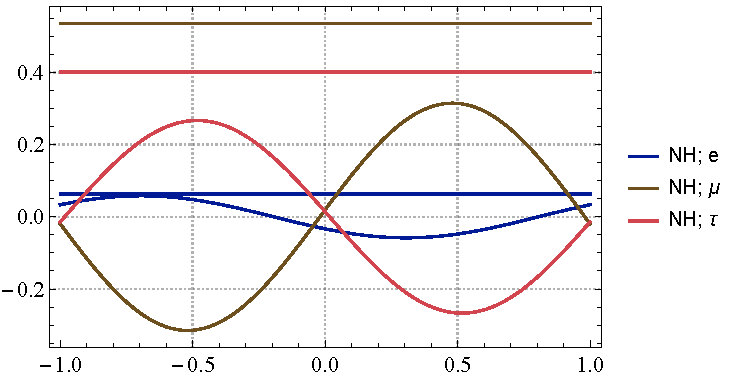
\includegraphics[width=0.49\textwidth]{bfp_analysis_f_NH.pdf}
  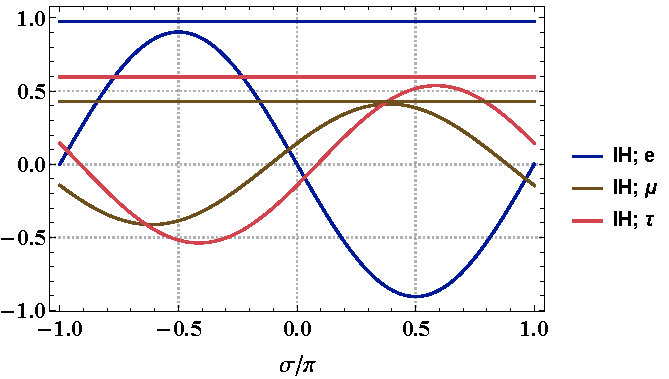
\includegraphics[width=0.49\textwidth]{bfp_analysis_f_IH.pdf}
\end{figure}

\subsection{Denominator}
Now we are to evaluate the denominator,
\begin{equation}
 D_\alpha := K_\alpha^{\text{eff}}\min(z_c, z_\alpha),
\end{equation}
where
\begin{align}
 z_\alpha &= 1.25\log25 K_\alpha^{\mathrm{eff}},&
 z_c &= \frac{M_1}{149\GeV},
\end{align}
and
\begin{equation}
 K_\alpha^{\mathrm{eff}}
= \kappa_\alpha \sum_I \frac{\Gamma_I}{H_N}\frac{|y_{I\alpha}|^2}{(yy^\dagger)_{II}}
= \kappa_\alpha \sum_I \frac{M_I|y_{I\alpha}|^2}{8\pi H_N}.
\end{equation}
We further evaluate it as
\begin{equation}
 K_\alpha^{\mathrm{eff}}
\approx\frac{M_1}{8\pi H_N} (y^\dagger y)_{\alpha\alpha}
\approx\frac{M_1^2}{4\pi v^2 H_N} 
\left(
U\w{PMNS}\sqrt{m}R^\dagger R\sqrt{m}U^\dagger\w{PMNS}
\right)_{\alpha\alpha},
\end{equation}
where we proceed as
\begin{align}
 K'_\alpha
&:=
\frac{2}{\mtot}\left(
U\w{PMNS}\sqrt{m}R^\dagger R\sqrt{m}U^\dagger\w{PMNS}
\right)_{\alpha\alpha}\\
&= G_\alpha^{(2)} \cosh2y -G_\alpha^{(1)}\zeta\sinh2y,\\
 K_\alpha^{\mathrm{eff}}
&\approx\frac{M_1^2}{4\pi v^2 H_N} \frac{\mtot}{2}K'_\alpha
=
\frac{m\w{tot}M\w{pl}}{8\pi v^2 \cdot 1.66\sqrt{g_*}}K'_\alpha.
\end{align}
As we see above, $K_\alpha'$ are $\Order(1)$-parameters; thus
\begin{equation}
 z_\alpha=1.25\log\frac{25m\w{tot}M\w{pl}}{8\pi v^2 \cdot 1.66\sqrt{g_*}}K'_\alpha\approx 10
\end{equation}
for both hierarchies, which is smaller than $z_c$ in the region of our interest.
Therefore, we evaluate the denominator as
\begin{align}
 D_\alpha\approx
\frac{1}{10}\cdot\frac{m\w{tot}M\w{pl}}{8\pi v^2 \cdot 1.66\sqrt{g_*}}\left(G_\alpha^{(2)} \cosh2y -G_\alpha^{(1)}\zeta\sinh2y\right).
\end{align}

\subsection{Total asymmetry}
Accordingly, as long as $R_{IJ}\ll 1$, i.e.,
\begin{equation}
 \delta M \gg  \frac{M_1\mtot}{16\pi v^2},
\end{equation}
we approximate the total lepton asymmetry as
\begin{align}
 \delta \eta_l&
\approx
\sum_{\alpha}
\frac{
  \frac{\rho_m\mtot}{2\pi v^2}\frac{M_1^3}{M_2^2-M_1^2}
  \frac{\cosh2y\sin2w}{\cosh^22y-\rho_m^2\cos^22w}
  \left[G^{(1)}_\alpha \zeta\cosh2y - G^{(2)}_\alpha\sinh2y\right]
}
{
  \frac{1}{10}\cdot\frac{m\w{tot}M\w{pl}}{8\pi v^2 \cdot 1.66\sqrt{g_*}}\left(G_\alpha^{(2)} \cosh2y -G_\alpha^{(1)}\zeta\sinh2y\right)
}
\\&=
-\frac{10\cdot1.66\sqrt{g_*}\rho_m}{M\w{pl}}
  \frac{4M_1^3}{M_2^2-M_1^2}
  \frac{\cosh2y\sin2w}{\cosh^22y-\rho_m^2\cos^22w}
\sum_{\alpha}
\frac{G^{(1)}_\alpha \zeta - G^{(2)}_\alpha\tanh2y}
{G_\alpha^{(1)}\zeta\tanh2y-G_\alpha^{(2)}}
\\&=
-C
  \frac{M_1^3}{M_2^2-M_1^2}
  K(z)
\sum_{\alpha}G_\alpha(z,\zeta),
 \end{align}
where
\begin{align}
 C &:= \frac{4\cdot10\cdot1.66\sqrt{g_*}\rho_m}{M\w{pl}}
\approx
\frac{4.0\EE{-17} ~~ (4.2\EE{-19})}{\text{GeV}}\quad\text{for NH (IH)},\\
 K(z) &:=   \frac{\cosh2y\sin2w}{\cosh^22y-\rho_m^2\cos^22w},
\qquad
G_\alpha(z,\zeta) :=\frac{G^{(1)}_\alpha \zeta- G^{(2)}_\alpha\tanh2y}
     {G_\alpha^{(1)}\zeta\tanh2y-G_\alpha^{(2)}}.
\end{align}
Here, $G_a(z,\zeta)$ depends on $U\w{PMNS}$ and $m_i$, while $K(z)$ has no dependence on $U\w{PMNS}$.
\section{(a few) Discussion}
We are interested in the lower bound on $M_1$.
The neutrino-option condition may compensate smaller $M_1$ by having larger $|y|$ as
\begin{equation}
 \cosh2y\simeq \frac{f(M_1)}{\mtot},
\end{equation}
but for larger $|y|$ the leptogenesis gets worse:
\begin{equation}
 K(z)\approx \frac{\sin2w}{\cosh2y},\qquad
G_\alpha(z,\zeta) \approx \sign y;
\end{equation}
thus, even with $|\sin2w|=1$ with normal hierarchy,
\begin{equation}
 |\delta \eta_l|
\approx C \frac{M_1^3}{M_2^2-M_1^2}\frac{1}{\cosh2y}
\approx \frac{8\pi v^2\cdot C \mtot}{f(M_1)^2}R_{IJ}.
\end{equation}
Restricting 
with numerical evaluation, this yields
\begin{equation}
 |\delta \eta_l|\approx 10^{-8}\left(\frac{M_1}{4.3~(8.5)~\EE5\GeV}\right)^6 R_{IJ}
\end{equation}
Therefore, leptogenesis provides a lower bound at, at least, $430\TeV$ ($850\TeV$) for NH (IH).

\appendix
\section{Yukawa products}
We use the Casas--Ibarra parameterization with $z=w+\ii y$ and $\zeta=\pm1$:
With 
\begin{align}
 y_{Ii}y^*_{Jj} &= \frac{2}{v^2}\sum_{ab}
\sqrt{M_I}R_{Ia}\sqrt{m_a}(U^\dagger)_{ai}
U_{jb}\sqrt{m_b}(R^\dagger)_{bJ}\sqrt{M_J},
\\
 (yy^\dagger)_{IJ} &= \frac{2}{v^2}\sum_{a}
\sqrt{M_I}R_{Ia}{m_a}(R^\dagger)_{aJ}\sqrt{M_J},\\
 (y^\dagger y)_{ij} &= \frac{2}{v^2}\sum_{abI}
U_{ia}\sqrt{m_a}(R^\dagger)_{aI}
M_I R_{Ib}\sqrt{m_b}(U^\dagger)_{bj}.
\end{align}
Regardless of the hierarchy, these Yukawa combinations are rewritten by


\end{document}
